\chapter{Implementation}
This chapter describes the technical aspects of this project. It will start with a high-level overview of the program. This is followed with issues that were faced during the development of the application. Finally, the features of the final implementation will be described, including the use of testing during development.

\section{Software and Libraries}

For this project, Ruby on Rails was used as the main language for implementation because of its versatility as a web application framework and its maintainability. The application is also compatible with the application it will be adapted with, Team Feedback. For charting and graphical visualisations, the charting library Chartkick was used due to its simplicity for creating graphs. To implement an OAuth connection between the application and GitHub for repository information, GitHub's own Octokit library was used to make API calls to GitHub. This was used to retrieve repositories that a user was a contributor to (both private and public) and the content of files in these repositories at different commits. The development environment used to develop the application was JetBrain's RubyMine IDE. 

\section{Infrastructure}

\subsection{Back-end Infrastructure}

The bulk of the project was in creating the algorithm and implementing the Gestalt pattern matching algorithm from scratch in Ruby (since there were no existing libraries using it). These elements were then connected to the GitHub endpoint, which provided the user and repository information. A simple front-end was then implemented to show visualisations of the metrics generated by the algorithm. The entire application uses a Model-View-Controller (MVC) architecture as it is the design pattern implemented by Ruby on Rails by convention. This design pattern divides the different responsibilities of a web application to easier, manageable sections. The front-end/views of the application is implemented using Embedded Ruby (ERB), which is a HTML file with extracts of Ruby to allow computation inside the views of the application. Figure \ref{fig:7} depicts a UML class diagram that shows a more in-depth view of the infrastructure of the application. 

\begin{figure}[h]
    \centering
    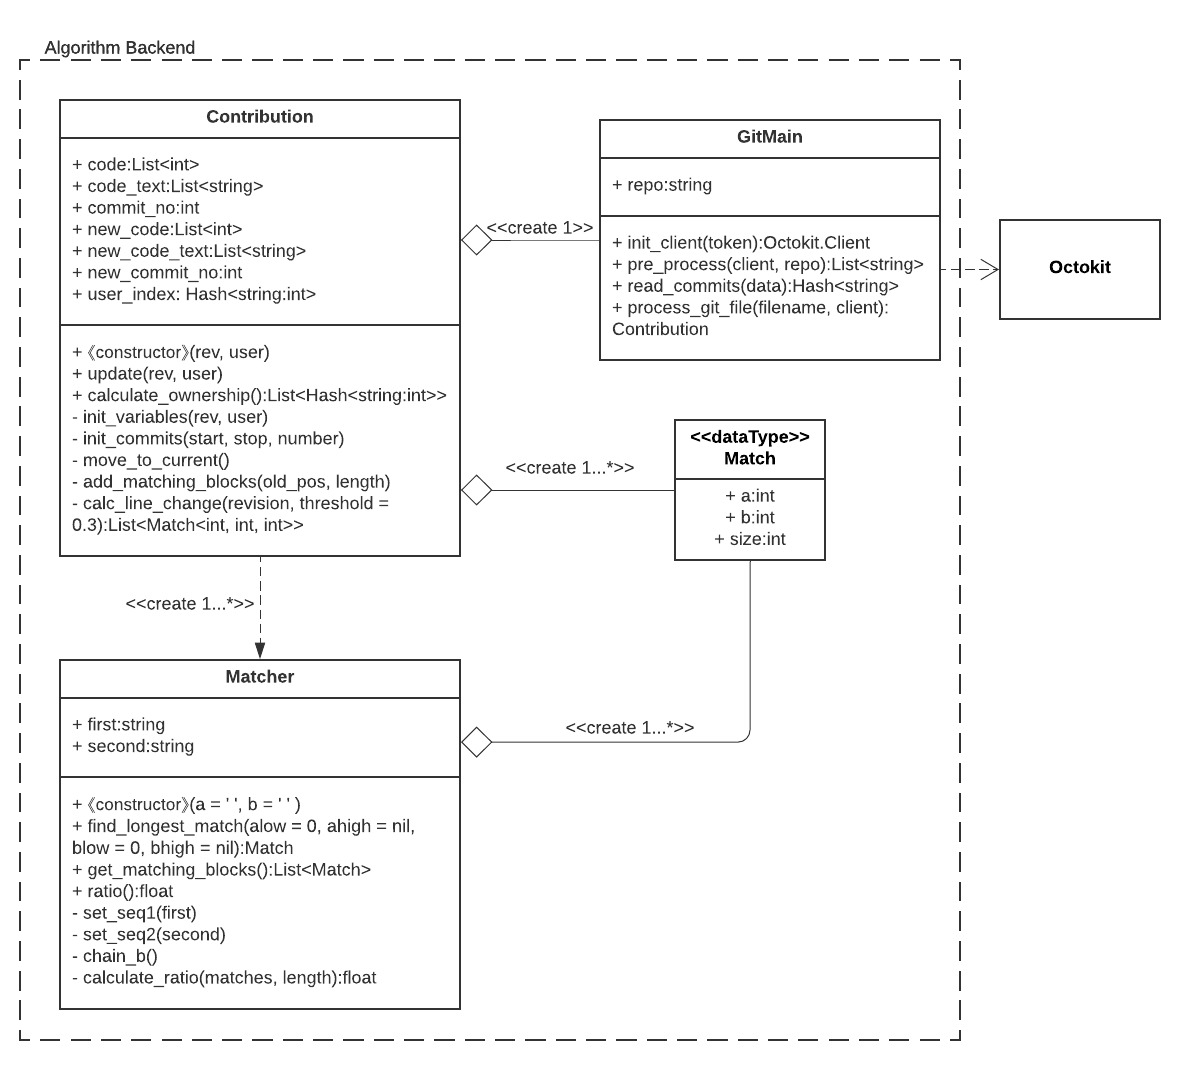
\includegraphics[scale=0.8]{images/UML class.jpeg}
    \caption{UML class diagram with a high-level overview of the application's back-end}
    \label{fig:7}
\end{figure}

The main components of the application's back-end can be seen above in Figure \ref{fig:7}. A brief description of each class can be seen below:
\begin{itemize}
    \item \textbf{Contribution}: The class containing the created algorithms that were discussed in Chapter 5 as Algorithm 1 and Algorithm 2.
    \item \textbf{Matcher}: The class that contains the Ruby implementation for the Gestalt Pattern Matching algorithm.
    \item \textbf{GitMain}: The class that implements the GitHub API calls for all the relevant repository required for the rest of the application.
\end{itemize}

\subsection{Front-end Infrastructure}

The front-end of the application is slightly more complex compared to the back-end as there are multiple views that utilise the Model-View-Controller (MVC) architecture as much as possible. The application starts off at a home page where the user is prompted to login using their GitHub account. If it is the user's first use of the application, they are then redirected to an external authorisation request from GitHub to allow the application to gain access to the user's basic profile details and their repositories. If the application is authorised by the user, the relevant controller retrieves the user's repository information and displays all of the user's repositories in a simple table. However, if the application is not authorised by the user, the user is redirected back to the home page. After the application is authorised, the user is then prompted to choose one of these repositories for analysis. When a repository is selected by the user, the application then queries the back-end of the application to get each file of the selected repository analysed by the \texttt{Contribution} class. Once the analysis is completed by the algorithms, the user is displayed with two different visualisations: a pie chart showing percentage contribution for each user, and a bar chart showing each user's persistence score. The view of this page also allows the user to change to some additional visualisations such as the ``Team View" and the ``File View".

When the ``Team View" button is clicked, the current page is reloaded to change the two visualisations from the original pie chart and bar chart to a more generalised version of these graphs. The currently logged in user would have their contributions compared to the rest of the team instead of each individual contributor. When the ``File View" button is clicked, a new page is displayed that lists all the files in the selected repository. The user can then click any of these files to get a new visualisation. This visualisation shows the selected file's contents at the most recent revision. The content of the file is then highlighted per character depending on the user that was attributed those changes by the algorithm. This gives the user a simple indication of how the algorithm works and allows the user to understand their contribution scores better.

In total, there are five different views for the application. The implementation of these views partially utilised the built-in CRUD (Create, Read, Update, Delete) routes for resources. For both the repositories list and the displaying of each repository's visualisations, the \text{Read} route mappings were utilised. For listing files in a repository and showing the file-based visualisation, the \texttt{Files} resource was set as a sub resource to the \texttt{Repos} to allow the file visualisation to be specific to each repository in the easiest implementation possible. Here, the \text{Read} route mappings were also utilised. The two \texttt{GET} routes utilised were \texttt{repos\#index} and \texttt{repos\#show} for both resources. Figure \ref{fig:8} shows the simple definition of the resources in lines 5-6.

\begin{figure}[h]
    \centering
    \begin{minted}[
    breaklines,
    frame=lines,
    framesep=2mm,
    baselinestretch=1.2,
    bgcolor=black,
    linenos]{ruby}
    Rails.application.routes.draw do
      root 'home#index'
      get 'home/index'
      get '/users/auth/github/callback', to: 'home#callback'
      resources :repos do
        resources :files
      end
    end
    \end{minted}
    \caption{Routes definitions in \texttt{routes.rb}}
    \label{fig:8}
\end{figure}

This meant that only 3 controllers were required for the entire application: \texttt{HomeController}, \texttt{ReposController} and \texttt{FilesController}. Below is the purpose of each controller:
\begin{enumerate}
    \item \texttt{HomeController}: Handle the callback route as defined in line 4 of Figure \ref{fig:8}. This callback route returns the authorisation code from GitHub and the controller carries out the exchange process discussed below in section 5.2.3 from step 4 to 5. Once the exchange is done, the user is redirected to the \texttt{repos\#index} view.
    \item \texttt{ReposController}: Handles both the \texttt{repos\#index} view and th \texttt{repos\#show} view. The \texttt{repos\#index} view displays a list of the user's repositories which is retrieved by the controller. The \texttt{repos\#show} view displays the visualisations specific to the selected repository. This controller is also responsible for converting the metrics produced for each file and amalgamating them to the data sets used for the ``Team" and ``Individual" visualisations. This involves accumulating the results for each file to a hash with a different key for each user.
    \item \texttt{FilesController}: Handles both the \texttt{files\#index} view and the \texttt{files\#show} view. It produces a list of the files in the selected repository for the \texttt{files\#index} view. For the \texttt{files\#show} view, the controller retrieves the selected file's attribution information from the \texttt{Contribution} algorithm, which is passed to the view to generate the highlighting of attribution for each user. 
\end{enumerate}

\subsection{GitHub integration}

The integration of GitHub accounts into the application was a complex process with many steps to get a user's authenticated information. Using the application as an authenticated user was essential for this application to have a higher API polling rate from 1000 requests per hour to 5000 requests per hour. One run-through of the application uses between 500 and 1000 API requests depending on the size of the repository so having this increased polling rate would allow the application to be run multiple times per hour. The process of authenticating a user is as follows:

\begin{enumerate}
    \item The user clicks on a Login button on the home page to start the authentication process. The link the user is sent to contains the client ID (which is created on the GitHub website) for the application and the requested scope of authorisation. 
    \item The button, when clicked, redirects the user to an external authorisation page on GitHub. This OAuth page requests for access to the user's personal user data and their public and private repositories for the application.
    \item If authorised, GitHub sends an authorisation code to the application. If unauthorised, the user is redirected to the home page.
    \item The authorisation code is then exchanged by the application for an access token using the application's client ID and client secret. This is done using one of the methods built into Octokit: \texttt{exchange\_code\_for\_token}. This method takes the authorisation code received from GitHub, the client ID and the client secret. It returns an access token which allows an \texttt{Octokit::Client} object to be created.
    \item The access is then passed from a temporary hash to a session variable. 
    \item The access token is passed into the constructor of the \texttt{Octokit::Client} class, which returns a \texttt{Client} object which can be used for all the API calls with the higher polling rate.
\end{enumerate}

\section{Testing and Verification}

As the application was being developed, branch testing was used extensively to ensure all branches were reached with the valid inputs needed for the branches to be reached. This type of testing was used mostly for verifying the algorithm and the many conditional statements used throughout the application. Branch testing was applied as each unit of the application was being developed, alongside verification tests to make sure these branches were both reached and returning the correct outputs. Once the application was at a working state and nearing completion, negative testing was employed to help identify any faults in the application. Erroneous data, such as empty files and new white space being added to files, were inputted to the algorithm using a benchmark data set (a GitHub repository with sets of erroneous files). \texttt{Begin-rescue} statements were used throughout the application to maintain the correct web flow for the application. An example of this is shown in Figure \ref{fig:9}, which occurs when the user does not authorise the application to their GitHub information.

\begin{figure}[h]
    \centering
    \begin{minted}[
    breaklines,
    frame=lines,
    framesep=2mm,
    baselinestretch=1.2,
    bgcolor=black,
    linenos]{ruby}
    def index
      ReposController.git = GitMain.new
      ReposController.client = ReposController.git.init_client(session[:access_token])
      begin
        @user = ReposController.client.user
        @profile_url = @user[:html_url]
        @user_name = @user[:name]
        @user_picture = @user[:avatar_url]
        @repos = ReposController.client.repos(access_token: session[:access_token])
      rescue Octokit::Unauthorized
        redirect_to '/'
      end
    end
    \end{minted}
    \caption{Error handling in \texttt{ReposController}}
    \label{fig:9}
\end{figure}

This example of error handling tries to initialise a \texttt{Octokit::Client} object in line 3 using the access token currently stored for this session. As previously discussed in Section 5.2.3, the access token is retrieved through an exchange process. If the user does not authorise the application, the exchange process still occurs but the process returns an unauthorised access token. This results a \texttt{Octokit::Unauthorized} exception to be thrown when a \texttt{Octokit::Client} object is created and attempted to be queried. When this occurs, the user is redirected back to the home page so they can authorise the application.

Unit testing was also heavily utilised for both the front-end and the back-end of the application in completing both branch and negative testing. An example of a unit test implemented in the application is \texttt{HomeControllerTest} as shown in Figure \ref{fig:10}. This test is a simple verification test to check the home page is reachable with a successful HTTP response code (200 - 299). 

\begin{figure}[h]
    \centering
    \begin{minted}[
    breaklines,
    frame=lines,
    framesep=2mm,
    baselinestretch=1.2,
    bgcolor=black,
    linenos]{ruby}
    require 'test_helper'

    class HomeControllerTest < ActionDispatch::IntegrationTest
      test "should get index" do
        get home_index_url
        assert_response :success
      end
    end
    \end{minted}
    \caption{Unit test in \texttt{HomeControllerTest}}
    \label{fig:10}
\end{figure}

\section{Maintainability}

Maintainability is a key feature to be considered when evaluating a software project. When developing the application, maintainability was one of the most important factors considered when making changes to the application. During the design of the application, it was important to keep the cohesion between modules in the application to be as high as possible. Coupling was also another characteristic that was considered at the design stage to keep this as loose as possible. Figure \ref{fig:7} clearly shows some of these considerations. It's clear to see from the class diagram that the application has minimal dependencies between each class/module (from the limited number of lines between each class). There is also a limited number of external dependencies since the pattern matching algorithm was coded from scratch and the GitHub integration only required one library to be installed, Octokit. This promotes loose coupling between modules and makes sure no module is over reliant to any other module. For example, no module relies on the overarching \texttt{Contribution} class. Additionally, attribute accessors (``getters") and mutators (``setters") were used to prevent implicit coupling and keep information regarding a class encapsulated. Reducing as many instances of coupling maximises an application's maintainability since each module can be reused and easily be tested independently. New modules can also be easily added to the application as there is no current dependencies within modules that need to be mimicked in new modules.

Figure \ref{fig:7} also demonstrates high cohesion within each module. Exemplar to this, each controller is concerned only with the views they are controlling. This is facilitated by the built in framework from Ruby on Rails to promote the Model View Controller design pattern. By default, the design pattern makes sure the views are separate from the logic of the application. This makes sure that the display and the data are able to change without affecting the other. One place the high cohesion is adamant is in the \texttt{FilesController}. Since the files retrieved for the \texttt{files/index} page depends on the selected repository, one could create an instance of the \texttt{ReposController} to have access to all the properties necessary for the view to be generated. However, this can give the class access to attributes that are not needed by it. Instead, \texttt{ReposController} defines attribute accessors that are needed by the \texttt{FilesController} and they are simply called by the class (as seen in Figure \ref{fig:11}). This helps eliminate any DRY (Don't Repeat Yourself) code for retrieving filenames.

\begin{figure}[h]
    \centering
    \begin{minted}[
    breaklines,
    frame=lines,
    framesep=2mm,
    baselinestretch=1.2,
    bgcolor=black,
    linenos]{ruby}
    def index
      @repo_name = ReposController.repo_name
      @files = ReposController.files
    end
    \end{minted}
    \caption{Logic for the \texttt{files/index} view in \texttt{FilesController}}
    \label{fig:11}
\end{figure}

Following coding style is another way to keep an application maintainable. If a large codebase has a high quality but follows no existing styling standards, the software becomes a difficult problem for maintaining in the future. For the application, RubyMine's built-in integration of The Ruby Style Guide \citep{batsov_2021} (using RuboCop) was integral in following these styling guidelines. These guidelines are very similar to and inspired by Python's PEP 8 style guide. One of the most important parts of the style guide is to use descriptive identifiers for all units of the application such as classes, methods and variables. An example of this in the application is \texttt{calculate\_ownership()} method in the \texttt{Contribution} class which calculates each user's separate contributions.